\documentclass[aspectratio=169,11pt]{beamer}
\usepackage[T1]{fontenc}
\usepackage{lmodern}
\usepackage{booktabs}
\usepackage{tikz}
\usetikzlibrary{arrows.meta,positioning,shapes.geometric,calc}
\usepackage{graphicx}
\usepackage{colortbl}

% ---------- look ----------
\definecolor{ink}{RGB}{28,36,52}
\definecolor{accent}{RGB}{214,96,0}
\definecolor{teal}{RGB}{0,121,140}
\definecolor{soft}{RGB}{242,244,247}
\definecolor{good}{RGB}{30,130,76}
\definecolor{bad}{RGB}{180,40,40}
\usetheme{default}
\setbeamertemplate{navigation symbols}{}
\setbeamercolor{normal text}{fg=ink}
\setbeamercolor{frametitle}{fg=ink}
\setbeamercolor{structure}{fg=teal}
\setbeamercolor{alerted text}{fg=accent}
\setbeamerfont{frametitle}{series=\bfseries,size=\Large}
\setbeamertemplate{frametitle}{\vspace{6pt}\insertframetitle\par\vspace{-2pt}{\color{accent}\rule{2.2cm}{2pt}}}
\setbeamertemplate{itemize item}{\color{accent}$\bullet$}
\setbeamertemplate{itemize subitem}{\color{teal}--}
\setbeamertemplate{footline}{\hfill{\color{gray}\scriptsize Transaction-Thieves \quad \insertframenumber\,/\,\inserttotalframenumber}\hspace{10pt}\vspace{6pt}}
\newcommand{\eps}{\varepsilon}
\newcommand{\bignum}[2]{{\color{#1}\fontsize{30}{32}\selectfont\bfseries #2}}
\tikzset{box/.style={draw=teal,very thick,rounded corners=4pt,fill=soft,align=center,font=\small,inner sep=5pt},
         ours/.style={box,draw=accent,fill=accent!10},
         arr/.style={-{Stealth[length=6pt]},very thick,color=ink!70}}

\begin{document}

% ---------- 1 title ----------
{\setbeamertemplate{footline}{}
\begin{frame}
\vspace{1.2cm}
{\fontsize{28}{32}\selectfont\bfseries Follow the Money\\[4pt] Without Moving the Data}\\[10pt]
{\color{teal}\large Privacy-limited questions between banks,\\ planned by an LLM agent, for anti-money-laundering}\\[16pt]
{\color{accent}\rule{4cm}{2pt}}\\[8pt]
Team \textbf{Cache me if you can}: Abhishek \textperiodcentered{} Bhavya \textperiodcentered{} Shreyas Deb \textperiodcentered{} Akshat Srivastava\\
{\small LMA Group Project 2026 \quad\textperiodcentered\quad \texttt{github.com/BhavyaV05/Transaction-Thieves}}
\end{frame}}

% ---------- 2 problem ----------
\begin{frame}{The problem: every bank sees only its own slice}
\begin{columns}[c]
\column{0.5\textwidth}
\begin{itemize}
\item Launderers route money \textbf{across banks} on purpose.
\item A model trained on one bank's view misses most of the pattern.
\item Banks \textbf{cannot pool data}. Legal sharing (US 314(b), MAS COSMIC) is slow, manual, and sends raw records.
\end{itemize}
\vspace{6pt}
\alert{\textbf{Our question:}} can a bank gain by asking other banks a few small, \emph{private} questions, without any record leaving them?
\column{0.48\textwidth}
\centering
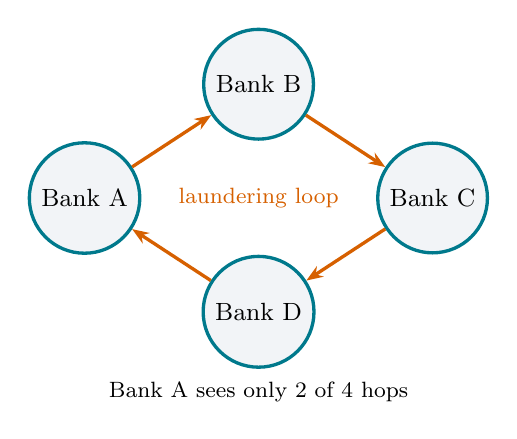
\begin{tikzpicture}[scale=0.85]
\foreach \x/\y/\n in {0/0/A,2.6/1.7/B,5.2/0/C,2.6/-1.7/D} \node[circle,draw=teal,very thick,fill=soft,minimum size=0.9cm] (\n) at (\x,\y) {\small Bank \n};
\draw[arr,accent] (A) -- (B); \draw[arr,accent] (B) -- (C); \draw[arr,accent] (C) -- (D); \draw[arr,accent] (D) -- (A);
\node[font=\footnotesize,color=accent] at (2.6,0) {laundering loop};
\node[font=\footnotesize,align=center] at (2.6,-2.9) {Bank A sees only 2 of 4 hops};
\end{tikzpicture}
\end{columns}
\end{frame}

% ---------- 3 idea ----------
\begin{frame}{The idea in one picture}
\centering
\resizebox{0.96\linewidth}{!}{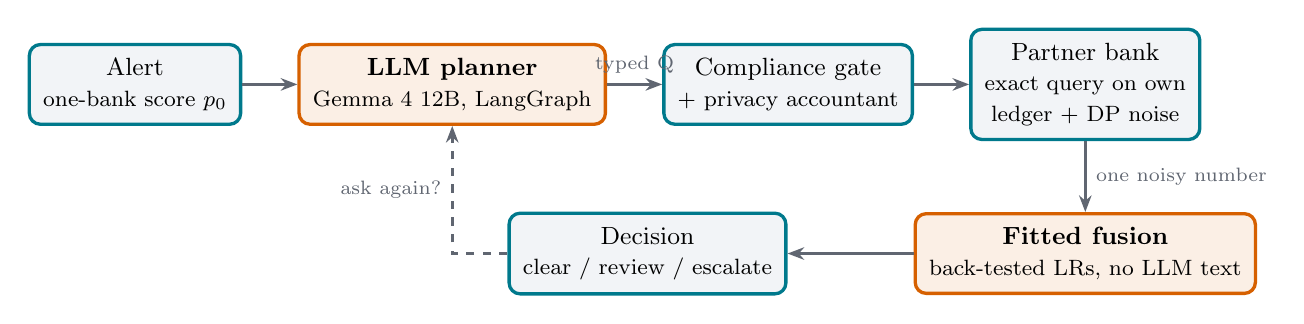
\begin{tikzpicture}[node distance=0.5cm and 0.7cm]
\node[box] (alert) {Alert\\{\footnotesize one-bank score $p_0$}};
\node[ours,right=of alert] (plan) {\textbf{LLM planner}\\{\footnotesize Gemma 4 12B, LangGraph}};
\node[box,right=of plan] (gate) {Compliance gate\\{\footnotesize + privacy accountant}};
\node[box,right=of gate] (bank) {Partner bank\\{\footnotesize exact query on own}\\{\footnotesize ledger + DP noise}};
\node[ours,below=0.9cm of bank] (fuse) {\textbf{Fitted fusion}\\{\footnotesize back-tested LRs, no LLM text}};
\node[box,left=1.6cm of fuse] (dec) {Decision\\{\footnotesize clear / review / escalate}};
\draw[arr] (alert) -- (plan); \draw[arr] (plan) -- node[above,font=\scriptsize]{typed Q} (gate); \draw[arr] (gate) -- (bank);
\draw[arr] (bank) -- node[right,font=\scriptsize]{one noisy number} (fuse);
\draw[arr] (fuse) -- (dec);
\draw[arr,dashed] (dec.west) -| node[near end,left,font=\scriptsize]{ask again?} (plan.south);
\end{tikzpicture}}
\vspace{8pt}
\begin{itemize}
\item \textbf{No transaction record leaves a partner bank}: only one number with differential privacy noise.
\item Budget $\eps = 2$ per alert, cap $\eps = 8$ per partner account. LLMs only see aliased accounts.
\end{itemize}
\end{frame}

% ---------- 4 three safeguards ----------
\begin{frame}{Three design rules that keep the LLM honest}
\begin{columns}[t]
\column{0.32\textwidth}
\centering\bignum{accent}{1}\\[2pt]\textbf{Back-test before trust}\\[4pt]
\raggedright\small Every question, even one the LLM just wrote, must prove on past alerts that its answer is informative (likelihood ratio + e-value FDR control).
\column{0.32\textwidth}
\centering\bignum{accent}{2}\\[2pt]\textbf{A formula decides}\\[4pt]
\raggedright\small The LLM plans. The final probability comes from $\operatorname{logit} p_0 + \sum w \log \mathrm{LR}$, numbers only. Prior work: an LLM investigator trusted its own reasoning and did \emph{worse} than its base model.
\column{0.32\textwidth}
\centering\bignum{accent}{3}\\[2pt]\textbf{One gate for everyone}\\[4pt]
\raggedright\small Our planner and every external agent use the same gate, accountant, simulated banks, backbone and call limits. Only the control loop differs.
\end{columns}
\end{frame}

% ---------- 5 data ----------
\begin{frame}{Data: IBM AMLworld, turned into 30 banks}
\begin{columns}[c]
\column{0.55\textwidth}
\begin{itemize}
\item \textbf{HI-Small} (5M transactions) for development, \textbf{HI-Medium} (32M) for the headline.
\item We built \textbf{30 bank views} with private ledgers, reply latency, declines and untrusted text notes.
\item \textbf{Time-respecting split}: days 1--9 / 10--12 / 13--16. Test split locked in code until the frozen final run.
\item \textbf{Conformal intake} passes only alerts the bank's model cannot settle.
\end{itemize}
\column{0.42\textwidth}
\centering
\begin{tabular}{lr}
\toprule
HI-Medium test & count \\
\midrule
Alerts & 4,478 \\
\quad headline period & 3,873 \\
\quad laundering & 975 \\
\alert{Askable} (a partner can answer) & \alert{\textbf{771}} \\
Random subset, askable & 208 \\
\bottomrule
\end{tabular}
\end{columns}
\end{frame}

% ---------- 6 what we built ----------
\begin{frame}{What we built and ran}
\begin{columns}[t]
\column{0.5\textwidth}
\textbf{\color{teal}Detection baselines (reproduced)}
\begin{itemize}\small
\item GFP + LightGBM: F1 62.95 vs 62.86 published
\item Multi-GNN (official code): F1 67.64 vs 68.16
\item MEGA-GNN (partial), FraudGT (500 epochs)
\item DP-FedAvg (Flower + Opacus), 6 $\eps$ levels $\times$ 3 seeds
\item Layer-wise exchange (Ceydeli et al.), 8 arms
\end{itemize}
\textbf{\color{teal}Planners compared}
\begin{itemize}\small
\item Random, fixed expert order, EIG, learned policy, enumerator of every question, raw record sharing
\end{itemize}
\column{0.5\textwidth}
\textbf{\color{teal}13 LLM agents ported into one harness}
\begin{itemize}\small
\item AML: Sharma, Torres, Co-Investigator, FinFRE-RAG
\item Info-seeking: BED-LLM, Uncertainty of Thoughts, debate
\item General: ReAct, Reflexion, ReWOO, LATS, LLMCompiler, DSPy-tuned ReAct
\end{itemize}
\textbf{\color{teal}Our LLM side}
\begin{itemize}\small
\item Backbone sweep of 7 open models (E18)
\item QLoRA student planner, 3 seeds (E16)
\item Qwen3-4B fast model with conformal cascade + injection screen
\end{itemize}
\end{columns}
\end{frame}

% ---------- 7 compute ----------
\begin{frame}{Compute: days of GPU time, one frozen test run}
\centering
\begin{columns}[c]
\column{0.24\textwidth}\centering\bignum{accent}{44}\\ GPU-hours\\{\footnotesize final test run alone (RTX 5070 Ti)}
\column{0.24\textwidth}\centering\bignum{accent}{$\sim$60}\\ GPU-hours\\{\footnotesize validation reruns on the LangGraph pipeline}
\column{0.24\textwidth}\centering\bignum{accent}{33}\\ systems\\{\footnotesize run on validation fit / cal / eval}
\column{0.24\textwidth}\centering\bignum{accent}{12k}\\ verdict rows\\{\footnotesize in the final run (GPU + CPU)}
\end{columns}
\vspace{8pt}
\begin{itemize}\small
\item Detection models trained for days on the 5070 Ti and a 3070 Ti laptop; RAG and injection benchmarks on the \emph{ada} HPC cluster.
\item Hypotheses H1--H10, thresholds and Holm order \textbf{pre-registered and frozen with a SHA-256 hash} before the test split was opened.
\end{itemize}
\end{frame}

% ---------- 8 metric ----------
\begin{frame}{How we score: gap closed}
\[
\text{gap closed} \;=\; \frac{B(\text{one bank}) - B(\text{system})}{B(\text{one bank}) - B(\text{see everything})}
\]
\vspace{4pt}
\begin{columns}[c]
\column{0.5\textwidth}
\begin{itemize}
\item $B$ = Brier score (lower is better)
\item \textbf{0} = no better than the bank alone
\item \textbf{1} = as good as pooling every bank's data
\item 95\% cluster-bootstrap intervals, Holm correction
\end{itemize}
\column{0.45\textwidth}
\begin{tabular}{lr}
\toprule
Detection model (3,873 alerts) & Brier \\
\midrule
GFP one bank & 0.1585 \\
GFP see everything & 0.0854 \\
\bottomrule
\end{tabular}\\[6pt]
{\small A big gap to close: precision in the top 10\% goes from 0.72 to 0.98.}
\end{columns}
\end{frame}

% ---------- 9 headline ----------
\begin{frame}{Headline: questions do not beat the bank alone}
\centering\small
\begin{tabular}{llrr}
\toprule
& System (771 askable test alerts) & Brier & Gap closed [95\% CI] \\
\midrule
Reference & One bank only & 0.1668 & 0 \\
& See everything (GFP) & 0.0966 & 1 \\
& Raw records from 3 banks, no privacy & 0.1640 & 0.040 [$-0.107$, 0.161] \\
\midrule
Non-LLM & Fixed expert order & 0.1694 & $-0.036$ \\
& Enumerator & 0.1708 & $-0.057$ \\
& Expected information gain & 0.1823 & $-0.220$ \\
\midrule
External & BED-LLM (best on validation) & 0.1956 & {\color{bad}$-0.410$} \\
\midrule
\alert{\textbf{Ours}} & \textbf{Compose, $\eps = 2$} & \textbf{0.1673} & $\mathbf{-0.007}$ [$-0.038$, 0.026] \\
\bottomrule
\end{tabular}
\vspace{8pt}
\begin{itemize}\small
\item Even \textbf{raw, noise-free} records close only 4\%: the limit is the data, not the privacy noise.
\end{itemize}
\end{frame}

% ---------- 10 hypotheses ----------
\begin{frame}{Pre-registered hypotheses on test}
\centering\small
\begin{tabular}{llrrl}
\toprule
& Hypothesis & Estimate [95\% CI] & $p_\text{Holm}$ & Verdict \\
\midrule
H1 & Gap closed vs one bank & $-0.007$ [$-0.038$, 0.026] & 1.00 & not supported \\
H2 & Benefit vs raw sharing & $-0.165$ [$-2.88$, 0.75] & 1.00 & not supported \\
H3 & LLM beats simple planners & $-0.001$ [$-0.006$, 0.003] & 0.33 & not supported \\
H4 & Back-testing helps & $-0.005$ [$-0.010$, $-0.000$] & 0.072 & not supported \\
\rowcolor{good!12}\textbf{H9} & \textbf{Beats best external agent} & \textbf{0.266} [$-0.022$, 0.799] & \textbf{0.004} & {\color{good}\textbf{supported}} \\
H7 & Formula vs LLM deciding & $-0.000$ [$-0.004$, 0.004] & 1.00 & not supported \\
\bottomrule
\end{tabular}
\vspace{8pt}
\begin{itemize}\small
\item H4 came close but its false-discovery audit failed. H5, H6, H8, H10 were not run in the reduced final plan.
\end{itemize}
\end{frame}

% ---------- 11 external ----------
\begin{frame}{Where we win: against published LLM agents}
\begin{columns}[c]
\column{0.56\textwidth}
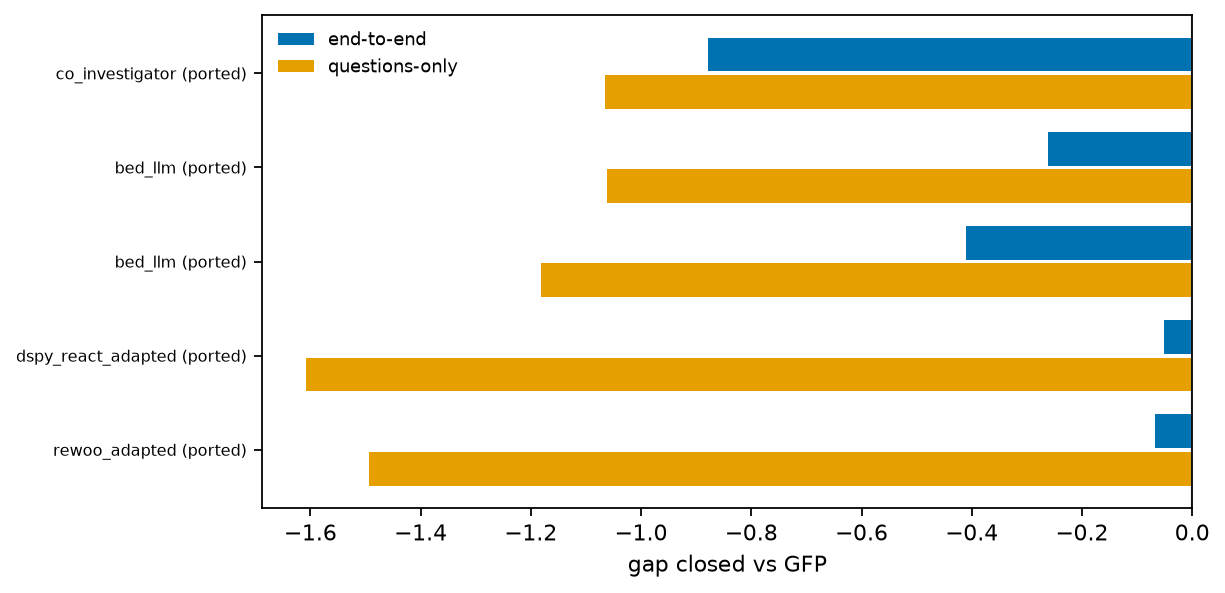
\includegraphics[width=\linewidth]{figures/external_gap.png}
\column{0.42\textwidth}
\small
\begin{tabular}{lr}
\toprule
Agent (208 subset) & Brier \\
\midrule
\textbf{Ours} & \textbf{0.1576} \\
DSPy ReAct (adapted) & 0.1623 \\
ReWOO (adapted) & 0.1638 \\
BED-LLM & 0.1805 \\
Co-Investigator & 0.2334 \\
\bottomrule
\end{tabular}\\[6pt]
\begin{itemize}\small
\item Agents that decide for themselves drift away from a well-calibrated $p_0$.
\item Co-Investigator gives no verdict on 71\% of alerts.
\item BED-LLM uses $3\times$ our LLM calls.
\end{itemize}
\end{columns}
\end{frame}

% ---------- 12 ablations ----------
\begin{frame}{Ablations: what earns its place}
\centering\small
\resizebox{\linewidth}{!}{\begin{tabular}{lrrl}
\toprule
Switch off (208 askable alerts) & Brier & $\Delta$ vs full [95\% CI] & \\
\midrule
Full system & 0.1576 & -- & \\
LLM may only pick from a fixed list & 0.1656 & +0.0080 [0.0031, 0.0131] & {\color{good}\textbf{composing helps}} \\
No back-testing & 0.1626 & +0.0049 [0.0003, 0.0099] & {\color{good}\textbf{back-testing helps}} \\
No stated hypothesis (act only) & 0.1592 & +0.0016 [$-0.0026$, 0.0059] & not significant \\
LLM decides stop / escalate & 0.1577 & +0.0001 [$-0.0035$, 0.0038] & no difference \\
\bottomrule
\end{tabular}}
\vspace{10pt}
\begin{itemize}\small
\item Without back-testing the agent asks \textbf{twice as many questions} and costs twice the GPU time, for a worse score.
\item From validation: naive fusion ($w = 1$) moved scores the wrong way (double counting $p_0$), so we fitted per-family weights.
\end{itemize}
\end{frame}

% ---------- 13 privacy + cost ----------
\begin{frame}{Privacy and cost}
\begin{columns}[c]
\column{0.5\textwidth}
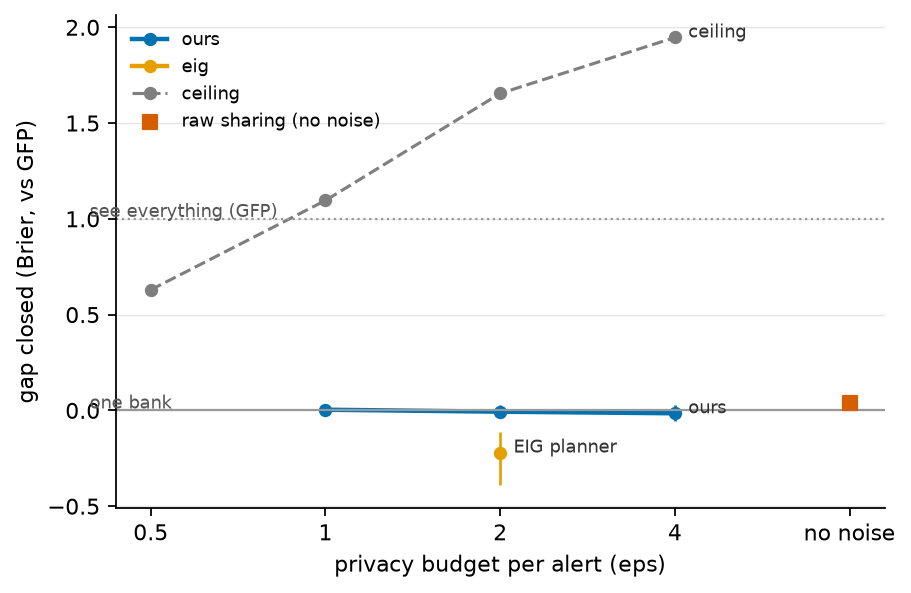
\includegraphics[width=\linewidth]{figures/privacy_curve.png}
\column{0.46\textwidth}
\begin{itemize}\small
\item Flat curve: $\eps = 1, 2, 4$ give Brier 0.1666, 0.1673, 0.1679.
\item Spends $\eps \approx 1.46$ of 2 per alert.
\item Per alert: \textbf{2.4 LLM calls}, 12.9k tokens, 29 GPU-seconds.
\item On all 3,873 alerts we \textbf{do no harm}: +0.0001 Brier vs one bank (BED-LLM +0.0057).
\end{itemize}
\end{columns}
\end{frame}

% ---------- 14 llm side ----------
\begin{frame}{The LLM side: backbone, fine-tuning, safety}
\begin{columns}[t]
\column{0.33\textwidth}
\textbf{\color{teal}Backbone sweep (E18)}\\[3pt]
\small 7 models, 2 stages. \textbf{Gemma 4 12B} won (0.1741 vs 0.1844 Qwen3.8-27B). ``Thinking'' mode spent its whole budget reasoning and was dropped.
\column{0.33\textwidth}
\textbf{\color{teal}QLoRA student (E16)}\\[3pt]
\small Qwen3-8B, LoRA r16, 3 seeds. Learned the format (token acc.\ 0.94) but planned worse than the 12B teacher (0.223 vs 0.201).
\column{0.33\textwidth}
\textbf{\color{teal}Fast model + safety}\\[3pt]
\small Qwen3-4B with conformal cascade: every error bound held. As an injection screen it cut ReAct's attack success from 5--8\% to \textbf{0\%}.
\end{columns}
\end{frame}

% ---------- 15 limitations ----------
\begin{frame}{Limitations and recorded deviations}
\begin{columns}[t]
\column{0.5\textwidth}
\textbf{\color{teal}Limitations}
\begin{itemize}\small
\item Synthetic data and simulated banks
\item Only $\sim$20\% of alerts are askable
\item Privacy per transaction, not per customer
\item Reduced final run: some arms not run
\end{itemize}
\column{0.5\textwidth}
\textbf{\color{teal}Deviations (all documented)}
\begin{itemize}\small
\item GFP see-everything rerun did not exactly reproduce; scores archived for a rerun
\item GNN official loaders leak future edges, so GFP is the only upper limit
\item CPU arms rerun with the frozen $p_0$; FraudGT scored before the freeze
\end{itemize}
\end{columns}
\end{frame}

% ---------- 16 conclusions ----------
\begin{frame}{Take-aways}
\begin{enumerate}
\item<1-> \textbf{Honest negative result.} Private questions between banks do not measurably beat a good one-bank model on AMLworld, and neither do raw records. The bottleneck is what a partner can add, not privacy.
\item<1-> \textbf{The safeguards work.} Back-testing plus a formula never hurts the base model, and it significantly beats published agents that let the LLM decide (H9).
\item<1-> \textbf{Inside the system}, composing new questions and back-testing them both measurably help.
\item<1-> \textbf{Reproductions} of GFP, Multi-GNN, MEGA-GNN and FraudGT on a time-respecting split, plus a finding that the GNN loaders leak future edges.
\end{enumerate}
\vspace{8pt}
{\color{accent}\rule{\linewidth}{1pt}}\\[4pt]
\centering\footnotesize Code, report and a README with full reproduction steps:\\ \texttt{github.com/BhavyaV05/Transaction-Thieves}
\end{frame}

{\setbeamertemplate{footline}{}
\begin{frame}
\centering\vspace{2cm}
{\fontsize{30}{34}\selectfont\bfseries Thank you}\\[10pt]
{\color{teal}Questions?}
\end{frame}}

\end{document}
